\documentclass[DM,lsstdraft,toc,usenatbib]{lsstdoc}

% Package imports go here
\usepackage{amsmath}	% Advanced maths commands
\usepackage{amssymb}
\usepackage{gensymb}  % degree symbol 
\usepackage{natbib}  % bibliography
\usepackage{cprotect} 
% Local commands go here

%% Journal abbreviations
%\bibliographystyle{aasjournal}

\title[Call for LSST Cadence White Papers]{Call for White Papers on \\ LSST Cadence Optimization} 

\author{\v{Z}eljko Ivezi\'{c}, Lynne Jones, Tiago Ribeiro, \\
                 the LSST Project Science Team, \\
                 and  the LSST Science Advisory Committee} 

\setDocRef{Document-XXX}
\date{\today}
\setDocRevision{v0.1}
\setDocStatus{draft}
\setDocAbstract{%
The LSST community is invited to play a key role in the definition of LSST's Observing Strategy 
by submitting white papers to help refine the cadence of observation in the `main survey' and 
fully define the use of the remaining 10\% of available time, distributed among a variety of `mini surveys'. 

The LSST Science Requirements Document (SRD) places minimal constraints on the observing strategy, 
recognizing that science evolves and that the initial (by now more than a decade old) survey strategy 
would have to be redefined closer to first light. With LSST first light expected in 2020, now is the time 
to undertake the final pre-commissioning planning for the initial LSST observing strategy. While
the existing candidate baseline survey strategy has been primarily defined by the LSST Project, the final planning
must be undertaken hand-in-hand with the community. 

<summary of what must be kept, what is open to change, how much time 10-20\%>
<combine white papers>

We are soliciting white papers to help plan these aspects of the LSST 
survey strategy. The deadline for these white papers is November 30, 2018.
}

% Change history defined here. Will be inserted into
% correct place with \maketitle
% OLDEST FIRST: VERSION, DATE, DESCRIPTION, OWNER NAME
\setDocChangeRecord{%
\addtohist{1}{2018-06-30}{First released version.}{\v{Z}eljko Ivezi\'{c}}
}

\begin{document}

% Create the title page
% Table of contents will be added automatically if "toc" class option
% is used.
\maketitle


\section{Introduction} 

The Large Synoptic Survey Telescope (LSST) will provide an unprecedented optical 
imaging dataset that will support investigations of our Solar System, Galaxy and Universe, 
across half the sky and over ten years of repeated observation. LSST observations will be
scheduled automatically, with the scheduling algorithm designed to address all science goals 
and maximize observing efficiency for given observing constraints (please see Appendix~\ref{sec:supp}
for a list of most relevant references describing LSST and its operations). LSST is constructing a 
flexible scheduling system that can respond to the unexpected and be re-optimized as the survey progresses.

Any implementation of LSST's 10-year observing strategy must meet the basic requirements described in the 
LSST Science Requirements Document (\href{http://ls.st/srd}{SRD}\footnote{The LSST Science 
Requirements Document (SRD) is available at \href{http://ls.st/srd}{http://ls.st/srd}})
for the core LSST science goals:
\begin{itemize}
\item constraining dark energy and dark matter,
\item taking an inventory of the Solar System,
\item exploring the transient optical sky, and
\item mapping the Milky Way.
\end{itemize}
However, in practice, the SRD intentionally places minimal quantitative constraints on the observing strategy,
primarily requiring:
\begin{itemize} 
\item A footprint for the `main survey' of at least 18,000 square degrees which must
obtain at least 825 visits per field (see SRD Tables 22 and 23), which places a minimum constraint on the time required to complete 
the main survey. Simulated surveys indicate this means that the main survey typically requires 85--90\% of the available time to 
reach this benchmark; even with scheduling improvements, it is unlikely that the goals of the main survey could be met with a time allocation
significantly below 80\%. 
\item Parallax and proper motion accuracies of 3~mas and 1~mas/yr at $r=24$, respectively (see SRD Table 26), which places
a light constraint on distributing visits throughout the lifetime of the survey and throughout a season.
\item Rapid revisits (40 seconds to 30 minutes) must be acquired over an area of at least 2000 square degrees (see SRD table 25) for
very fast transient discovery; this requirement can usually be satisfied via field overlaps when surveying contiguous areas of sky. 
\end{itemize}
This leaves significant flexibility in the detailed cadence of observations within
the main survey footprint, including the distribution of visits within a season (or between seasons), the distribution between filters and 
the definition of a `visit' itself. Furthermore, these constraints apply to the main survey, which is expected to
require at most 90\% of the observing time; the use of the remaining time in mini surveys is not constrained in the SRD.

A brief introduction to the current candidate baseline survey strategy, expanded background of the primary LSST science 
goals, and concise descriptions of how these goals drive the basic survey strategy and data processing
requirements are provided in the \href{http://ls.st/pif}{LSST Overview paper}\footnote{The LSST Overview 
paper is a living document available at \href{http://ls.st/pif}{http://ls.st/pif}.}.
This current candidate baseline survey strategy, as represented in the reference survey simulation, includes the main survey and
several candidate mini surveys (for more details, please see Appendix A): 
\begin{itemize}
\item The {\bf main ``wide-fast-deep'' survey}, which covers $\sim$18,000 deg$^2$ of sky within equatorial declination
range $-62^\circ < \delta < +2^\circ$, and excluding the central portion of the Galactic 
plane. Within the main survey, two visits\footnote{A `visit' here is an LSST default visit, which 
consists of back-to-back 15 sec exposures, for a total of 30 sec of on-sky exposure time. These back-to-back exposures are always
in the same filter, separated only by the 2 second readout time.} 
per field (in either the same or different filters) are acquired in each night, to allow identification of moving objects, rapidly varying transients, and improve
the reliability of the alert stream. These pairs of visits are repeated every three to four nights throughout the period the field is visible in each year. Each
field in the main survey receives about 825 visits throughout the ten years of the LSST survey, spread over the six LSST filters 
$ugrizy$. The quantitative SRD constraints on area coverage, number of visits, parallax and proper motion errors, and 
rapid-revisit rate (40 seconds -- 30 minutes) apply to visits obtained in the main survey. 
In the current reference simulation, the main survey uses 86.4\% of the available time.
\item The {\bf North Ecliptic Spur candidate mini survey} covers the area north of $\delta = +2^\circ$ to $10^\circ$ north of the Ecliptic plane
and is intended to observe the entire Ecliptic plane for purposes of inventorying the minor bodies in the Solar System. This area ($\sim$ 4160 deg$^2$) 
is observed on a schedule similar to the main survey, although with a smaller total number of visits per field and only in filters $griz$. 
As implemented in the current reference simulation, the North Ecliptic Spur mini survey uses about 5.5\% of the available time. 
\item The {\bf Galactic Plane candidate mini survey} covers the central portion of the Galactic plane which is not included in the main survey, 
centered around $|l| = 0^\circ$ and covering $\sim$ 1860 deg$^2$.  It is observed at a much reduced rate compared to the main survey, 
and with a smaller total number of observations per field (30 visits per field and per filter, in $ugrizy$), so as to
provide astrometry and photometry of stars toward the galactic center but without reaching the confusion limit of the coadded images.
There is no requirement for pairs of visits in each night in this area. As implemented in the current reference simulation, the Galactic Plane mini survey uses
about 1.6\% of the available time.
\item The {\bf South Celestial Pole candidate mini survey} covers the region south of the main survey, to the South Celestial Pole, $\sim$ 2315 deg$^2$,
including the Magellanic Clouds. 
This mini survey is observed with a strategy similar to the Galactic Plane mini survey, with 30 visits per field per filter in $ugrizy$, 
and without requiring pairs of visits. This provides coverage of the Magellanic clouds, but without committing extensive time as these fields are
at high airmasses from the LSST site. As implemented in the current reference simulation, the South Celestial Pole mini survey uses
about 2.0\% of the available time.
\item The {\bf Deep Drilling Field candidate mini survey} is implemented as five specific field pointings $\sim$ 50 deg$^2$, 
which are observed with a much denser sampling rate. These fields
are observed every three to four days, but in a sequence of multiple $grizy$ exposures during gray and bright time, and then
multiple sequential $u$ band exposures during dark time. The current deep drilling fields are aimed at extragalactic
science, providing a `gold sample' to calibrate the main survey, and to discover Type Ia supernovae. 
As implemented in the current reference simulation, the Deep Drilling Fields mini survey uses about 4.6\% of the available time.
\end{itemize}

Due to the desire for multi-wavelength precursor observations for the deep drilling fields, and the limited lifetime of relevant 
space-based observatories, the locations of four of the Deep Drilling fields have been finalized, while any remaining field locations 
have yet to be specified. The locations of these four deep fields were announced in 2012, as the result of a community driven process 
with the goal of obtaining multi-wavelength
coverage by ground and space-based facilities some of which may not exist at the start of the LSST survey.
These fields are intended to coincide with multi-wavelength surveys targeting the ELAIS-S1, XMM-LSS, Extended Chandra Deep Field-South, 
and COSMOS pointings. The cadence of observations within these (or any) deep drilling fields is not finalized, although the coadded
depth may be expected to be at least one magnitude deeper than the LSST main survey in each filter.

Beyond the SRD constraints and commitment to the four deep drilling fields, the survey strategy as implemented in the candidate baseline 
above should not be considered guaranteed, and candidate mini surveys present in the current baseline may not be carried forward to
the initial operations survey strategy; for illustrative examples of some alternate survey strategies, please see Appendix~\ref{sec:surveys}.
All of the candidate mini surveys and the cadence in the main survey will be re-evaluated on the basis of community input in the next 
step of planning for the initial LSST survey strategy. Much of the existing survey strategy 
has been based on a mix of community and project input, but the overall balance has been project-driven. 
The detailed cadence of visits in the main survey, the footprint for any other mini survey (except the location of the four pre-announced 
deep drilling fields), and the cadence or number of visits in any mini survey are open topics for optimization. 
The main purpose of this call for white papers is to solicit detailed input from the community interested in 
LSST science in order to design the optimum overall survey strategy. 


\subsection{The LSST Community Observing Strategy Evaluation Paper (COSEP): ongoing community feedback}

The LSST community is already playing a key role in the refinement of LSST's observing strategy 
by developing and analyzing metrics for quantifying the performance of simulated surveys generated by
the LSST project.  This work is being assembled in an open github community\footnote{
https://github.com/LSSTScienceCollaborations/ObservingStrategy}, 
in the form of a large cross-community survey evaluation paper
titled \href{http://ls.st/9fw}{`Science-Driven Optimization of the LSST Survey Strategy'}\footnote{The first 
version of this community observing strategy evaluation paper was published as arXiv:1708.04058 in August 2017.},
which will be referred to here as the Community Observing Strategy Evaluation Paper (COSEP). 
Chapter 1 and 2 of the COSEP provide a useful overview of the considerations involved in 
modifying the LSST survey strategy, as well as more details of the baseline survey strategy and 
examples of some possible variations in survey strategy, implemented in various simulated surveys.

The COSEP explores the effects of relatively small changes to the LSST survey strategy
on the detailed performance of the anticipated science investigations. The main lessons 
learned from the first version of this paper are: 
\begin{enumerate} 
\item The LSST Project should simulate, analyze and optimize the rolling cadence idea
(a non-uniform sampling in time in the wide-fast-deep survey designed to increase the frequency of 
observations for better coverage of variable phenomena on time scales of a few months, driven 
by supernovae, asteroids, and short-timescale stellar variability, at the cost of decreasing the 
frequency slightly at other times), and 
\item The LSST Project should execute a systematic effort to further improve the ultimate
LSST survey strategy (e.g., sky coverage optimization, u band depth optimization, mini surveys). 
\end{enumerate} 

Through the end of construction and commissioning, the COSEP will remain a living document 
and the main vehicle for the community to broadly communicate to the LSST Project regarding 
the scientific repercussions of various observing strategies. It will serve as a repository
of metrics, with performance evaluations of existing simulated surveys. Periodically, the LSST
Project Scientist, with support from the Project Science Team (PST) and the Science Advisory Council (SAC), 
will review these metrics and evaluations, to fold updates into the survey optimization efforts.

While the COSEP will continue to provide the means to update evaluations of the survey strategy, the white 
papers solicited in this call are intended to provide the LSST science community with an opportunity 
to propose more significant, detailed, modifications of the LSST survey strategy, including broad changes in
the mini surveys.

We anticipate the performance evaluation components of the white papers solicited here will also be added to the COSEP, to
provide a comprehensive reference point for survey strategy evaluation. 

\subsection{Motivation for this white paper call}

Guided by the community input summarized in the COSEP and further 
advice from the Science Advisory Committee (SAC), the LSST Construction Project has decided to
solicit detailed technical white papers for specific modifications of the current baseline survey strategy.

As discussed in more detail in Appendix A, analysis to date indicates that the baseline candidate
survey strategy, while meeting the basic science requirements for the LSST survey, can be meaningfully 
improved\footnote{The current, as-simulated, baseline survey strategy is described in detail in Sections 1.1 
and 2.3 in the \href{http://ls.st/o5k}{COSEP}.}
The LSST \href{http://ls.st/srd}{SRD}
provides minimal constraints on the survey strategy details because it recognized that science evolves and that the 
initial, by now more than a decade old, survey strategy will have to be re-optimized closer to first 
light. With LSST first light expected in 2020, now is the time to undertake the final pre-commissioning
optimization\footnote{``Optimization'' used here does not imply its strict mathematical meaning. 
We are attempting to create the best survey strategy possible, but this is not a formal optimization 
effort of an objective function in part because the concept of an ``optimized'' survey depends in part on a subjective
weighting of different science goals.} 
of the LSST baseline observing strategy. We seek science-driven input for cadence 
properties such as per-bandpass imaging depth, the sky coverage, temporal coverage, observing
rules, etc., as summarized in Appendix A. Investigations of a limited number of such survey strategy 
modifications are reported in Chapter 2 from the COSEP (and discussed 
in various supplementary materials listed in Appendix C). 


\subsection{General guidelines} 

We solicit detailed white papers for specific modifications of the current baseline survey strategy, including 
both the main survey and the so-called ``deep drilling fields'' and other mini surveys. There are no 
specific limitations on what kind of science programs will be considered, but please note that 
the primary four LSST science themes remain the cornerstones of the LSST survey and must be
maintained. Indeed, the LSST SRD states that ``the adopted observing 
strategy will not jeopardize the goals of any of the four main science themes''. Each white paper should
include detailed metrics to evaluate the scientific performance and impact of the suggested changes; these metrics
do not need to be comprehensive across all science use cases\footnote{The LSST Project will provide metrics to evaluate
the SRD-required quantities, as well as run a combination of metrics contributed by the general science community to cover a 
wide range of science goals.}.

The detailed cadence of visits in the main survey, the footprint for any other mini survey (except the location of the four pre-announced
deep drilling fields), and the cadence or number of visits in any mini survey are open topics for optimization. The existence of a 
particular survey strategy for a given mini survey in the current baseline should not be taken to imply that it will be present in the same way in the final 
survey strategy. Metrics which support a given mini survey, and the accompanying science justification 

Detailed white papers are also solicited for novel ideas, such as twilight observing (see Appendix~\ref{sec:twilight}), 
as well as synergies with other major surveys ({\it e.g.}, WFIRST, Euclid). In addition, white papers for programs
which leverage LSST's unique large \'{e}tendue are more compelling than {\it e.g.,} single object investigations.  
At this time we are not soliciting proposals to optimize observations during the commissioning period.
%A call for commissioning proposals will be issued once the start date of commissioning is known with adequate accuracy (1-2 months). 

Technical constraints imposed by the system and observing conditions are summarized in 
Appendix B. If a proposed dataset will require special processing, a plan to obtain necessary software and compute resources 
must be provided in the white paper. In cases that require more detail, or in case of specific questions not addressed in this 
document, please start a discussion at \href{http://community.lsst.org}{community.lsst.org}\footnote{\url{https://community.lsst.org/c/sci/survey-strategy}}.

The LSST Science Requirements Document states that ``the adopted baseline design assumes a 
nominal 10-year duration with about 90\% of the observing time allocated for the main LSST survey.'',
and further clarifies that ``The remaining 10\% of observing time will be used to obtain improved 
coverage of parameter space\dots''. While the detailed time allocation will eventually depend on currently unknown system
performance parameters, it is unlikely that the goals of the main survey could be met with a time allocation
significantly below 80\%. In other words, it is plausible that the time allocated to programs other
than the main survey could significantly exceed 10\% (perhaps by as much as a factor of two), but 
no firm commitments beyond this statement of plausibility can be made at this time. 

The data from any given specialized survey will be treated in exactly the same way as all LSST 
data: there is no special proprietary access for any subset of the data from LSST. Indeed, the final set of the so-called
deep-drilling fields and other mini surveys may be based on an amalgam of ideas from different 
white papers; there will be no sense in which a survey strategy described in a given white paper must be accepted or rejected as-is.  


\subsection{Review process and timeline}

The deadline for submitting white papers is November 30, 2018. For submission instructions, 
please see the next section. 

Soon after the November 2018 submission deadline, members of the LSST Science Advisory Committee (SAC), 
with technical support from the Project, 
will triage the submitted white papers and decide which meet the criteria of scientific excellence and 
technical feasibility for further analysis (including suggestions for combining 
submitted ideas into single programs, and giving suggestions for maturation of the current notional 
extragalactic observing strategy). These criteria are discussed in Section~\ref{sec:ranking}. 

The input from the submitted white papers will be used to design multiple
options in observing strategies and a Project team will generate 
simulated surveys based on these survey strategies. 
These multiple simulated surveys will address varying science drivers and will form a 
``menu'' of possible survey strategies (e.g., a main 
survey with 18,000 deg$^2$ of sky coverage vs. sky coverage of 23,000 deg$^2$ to a
somewhat shallower depth). The performance evaluation criteria submitted as part of the 
white papers and in the COSEP will be used to generate quantitative assessments to compare these strategies. 

We anticipate that the list of observing strategies that will be simulated and analyzed 
(the ``menu'' above) will be available by April 2019. Simulated survey outputs and Metric Analysis 
Framework (MAF\footnote{https://sims-maf.lsst.io}) analyses will become available by the end 
of 2019. 

An advisory report on these survey strategies will be prepared by the Project for the LSST SAC during early 2020, 
in a close collaboration between the Project and the Observing Strategy Github community and 
LSST Science Collaborations. The SAC will in turn advise the Project on the specific survey strategy 
to be used at the start of full LSST operations, as well as on guidelines for the strategy throughout all ten years of the survey. 
In developing their recommendations to the Director, the SAC will be guided by selection 
criteria set by the Project Science Team and discussed in Section~\ref{sec:ranking} ({\it e.g.}, restrictions 
based on technical criteria, such as those discussed in Appendix B). The Director can further consult with the Project Science 
Team about the SAC survey strategy recommendations. A baseline simulation that reproduces the
adopted strategy, and its detailed performance analysis, will be published in 2021. 
The start of LSST operations is anticipated in 2022.

An overall aim of the Project and all stakeholders is to make this process transparent to the community and to base 
all decisions on quantitative input and pre-defined criteria to the maximum extent possible. 
The Project will organize a dedicated session at the LSST 2018 All-hands meeting (Tucson, Aug 13-17)
about this call for white papers, to further clarify  details, exchange ideas, discuss simulated surveys, 
and coordinate teams that plan to submit white papers. 


\section{White paper submission guidelines} 


\subsection{Who can submit a white paper?} 

All members of the scientific community interested in LSST science can submit a white paper. 
We reiterate that the data from any given specialized survey will be treated exactly the same 
way as all LSST data: the authors of white papers will have no proprietary access to it. There will be no 
formal ``acceptance'' of proposed ideas; with the overall ranking priority advice provided to the 
Project by the Science Advisory Committee, the Project Team will implement a number of
different strategies that will be used as quantitative input (``a menu of options'') by the 
Science Advisory Committee when recommending strategy for the initial phase of the LSST survey. 


\subsection{Requested input \label{sec:reqinput}}

The current baseline survey strategy (as represented in the reference survey simulation) includes:
\begin{itemize}
\item the main Wide-Fast-Deep (WFD) survey,
\item Northern Ecliptic Spur (NES) mini survey, 
\item Galactic Plane (GP) mini survey,
\item South Celestial Pole (SCP) mini survey, and
\item the Deep Drilling (DD) fields mini survey,
\end{itemize}
Quantitative, science-driven optimization input is requested for all of the above, as well as 
for survey strategy questions such as optimal visit exposure time,
co-added per-bandpass imaging depth, the sky coverage, temporal coverage, observing
rules, etc.  For a detailed discussion, please see Appendix A. The existence of a particular
mini survey, sequence of observations, or exposure time in the current baseline does not 
guarantee its existence in the same form in the final survey strategy. 

In addition to existing surveys listed above, we also seek input on new mini survey ideas 
to replace and/or enhance the current programs, including special ``Target of Opportunity'' (ToO) 
programs. We also solicit novel ideas, such as twilight observing (see Appendix~\ref{sec:twilight}),
as well as observing synergies with other major surveys (e.g., WFIRST, Euclid). 

We reiterate that that the observing time allocated to {\bf all} the mini surveys 
(including DD fields) is ``about'' 10\%, and is unlikely to exceed 20\% of the total available
observing time. We note that implementation details for mini surveys (especially DD fields)
are coupled at some level to the main survey: more time for the former means less 
for the latter, and some of the design decisions for the latter affect the science
case for the former.  For example, some rolling cadence strategies for the main survey  
may allow some variable and transient science to happen that would otherwise be the 
focus of a deep drilling field, and changes in the main survey footprint will affect the 
definition of a Galactic Plane survey. The Project will provide additional alternative 
survey simulations with this call for white papers to help illustrate some of these potential 
crossovers. 

\subsection{TeX template for submission \label{sec:textemplate}} 

Each proposed modification of the survey strategy must contain a Scientific Motivation, Technical Description, and Performance Evaluation section, instructions for which are expanded in the white paper submission template. The Scientific Motivation section is intended to explain why this survey strategy modification is important and what can be learned if the proposed observations were obtained, relative to some baseline. The Technical Description section details what observations are being requested and should provide enough detail to enable proper simulations\footnote{For more information on how survey simulations are created, please see the documentation on OpSim at \href{http://sims-opsim.lsst.io}{http://sims-opsim.lsst.io}.} to be created, as well as additional information that can help in the process of combining similar but separate survey strategy modification requests. The Performance Evaluation section must contain methods to evaluate the effectiveness of the survey strategy modifications, particularly in light of the potential effect of survey strategy changes proposed in other white papers. It is unlikely that any proposed cadence modification suggested in white papers will be carried out in its ``ideal'' form; thus metrics (along with threshold values for these figures of merit) to evaluate the science performance of non-ideal simulations are crucial. The TeX submission template should help with further instructions for each of these areas.

The submission template requests each white paper to self-assign to one of the following categories:
\begin{itemize} 
\item a specific observing strategy to enable specific time domain science, 
	that is relatively agnostic to where the telescope is pointed (e.g., a science case enabled 
	by relatively deep precise time-resolved multi-color photometry). 
\item a specific pointing or set of pointings that is (relatively) agnostic of the detailed observing 
	strategy or cadence, (e.g., a science case enabled by very deep precise multi-color 
	photometry)
\item an integrated program with science that hinges on the combination of pointing/detailed 
	observing strategy combination (e.g., search for variable stars in the 
	LMC/SMC). 
\end{itemize}  
If a specific white paper does not fit any of these categories, please state so.

The submission template and an example of the submission, with instructions about
all the required information, can be found in the git repository hosted at \href{https://github.com/lsst-pst/survey_strategy_wp}{lsst-pst/survey\_strategy\_wp}\footnote{\url{https://github.com/lsst-pst/survey_strategy_wp}}.
The submission process includes the following steps: 
%
\begin{enumerate}
\item Fork the repository using your (the PI's, or a selected collaborator's)  Github account.
\item Clone the forked repository to your local machine.
\item Create a directory with the PI name as LASTNAME\_FIRSTNAME\_NUMBER,
where NUMBER is a counter for multiple white papers submitted by the same person (or the case
of two people with the same name). 
\item Copy the template to the directory created in the last step.
\item Fill the latex template file with the white paper information. It is possible to make intermediate 
          commits to keep track of the changes to the white paper and share it with collaborators.
\item Once the proposal is ready, make a Pull Request (PR) to the master branch of the main repository. 
\item A team member will accept your PR, or contact you in case of problems. 
\end{enumerate}

For additional help or questions, please ask on \href{https://community.lsst.org/c/sci}{LSST Community}\footnote{\url{http://community.lsst.org/c/sci}}. 


\section{White paper ranking criteria \label{sec:ranking}} 

The ultimate LSST observing strategy will aim to deliver a cutting-edge data set to enable
the four LSST's cornerstone scientific programs, while at the same time maximizing the 
science possible with specialized observing using about 10\% of the total observing time. 

We anticipate that the adopted observing strategy will be based on an amalgam of ideas from 
different white papers; therefore, there will be no formal ``acceptance'' or ``rejection'' of
proposed ideas. The overall ranking priority advice provided to the Project by the Science Advisory Committee 
will be based on the following considerations: 
\begin{itemize}
\item {\bf Science} Importance and robustness of the proposed science program, including 
           its match to the unique abilities of the LSST system, and its consistency with the 
           main four LSST science themes. This could be a single strong science goal, synergies with
           other astronomical facilities, or a multitude of science goals enabled by the same survey strategy. 
\item {\bf Feasibility} Programs must be feasible from the hardware and software point of view (see Appendix B),
         specifically including any special data processing required. The complexity of the program, in terms of additional
         requirements on hardware and software beyond the baseline requirements, will also be considered. 
         The Project Science Team will conduct a technical check on submitted white papers.
\item {\bf Time requested} The amount of time (including overheads) required should be justified by 
        the associated science. 
\end{itemize} 

As always, the science program properties such as importance and robustness are open
to interpretation. It is inevitable that some science drivers will be in conflict, and even
observing efficiency may not be defined in an absolute sense. The Project and the Science Advisory 
Committee will strive to make the white paper ranking process transparent to the maximum extent possible. 


\vskip 0.2in 
{\it Acknowledgments:} this document has greatly benefited from discussions between 
the LSST Project Science Team, the LSST Science Advisory Committee and Kem Cook, 
Phil Marshall, Steve Ridgway, Daniel Rothchild, Peter Yoachim and numerous other members 
of the LSST Science Collaborations. 

\newpage
\appendix
\section{Examples of open survey strategy optimization questions \label{sec:optimization}} 

The quantitative optimization of the LSST observing strategy requires many 
detailed decisions to be made, often with only an indirect science justification,
or with conflicting science drivers.  The current most significant open questions and associated 
tradeoffs are listed below for the main survey and each mini survey. White papers are specifically 
encouraged to address these questions.

\begin{figure}[htb]
\centering
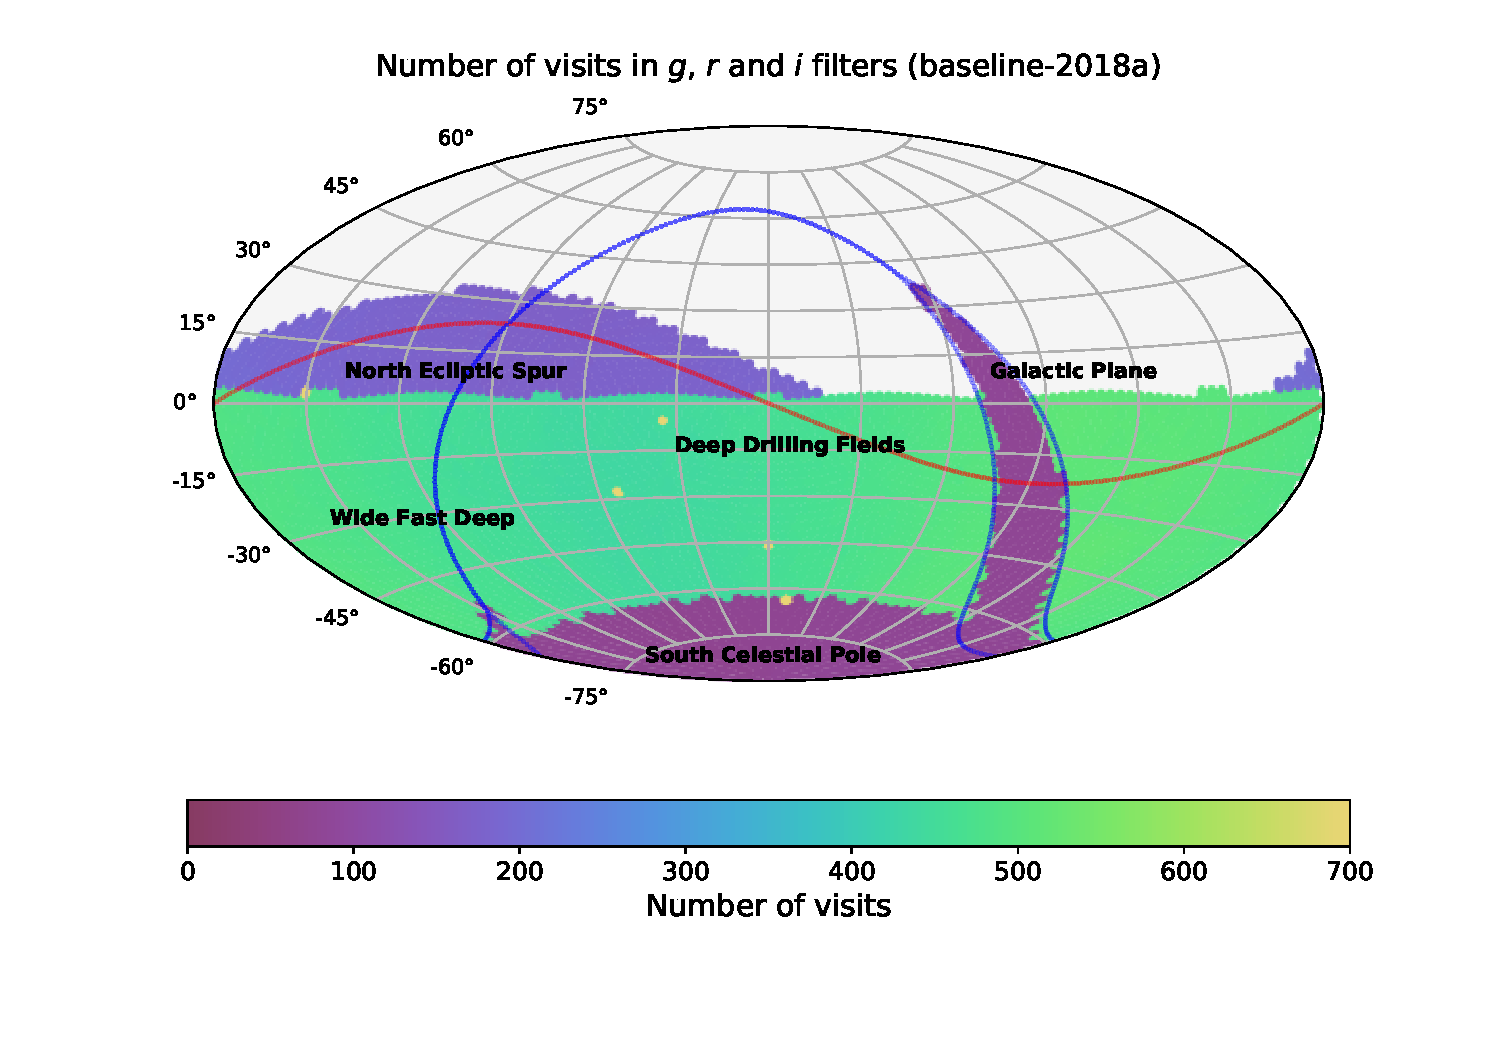
\includegraphics[width=0.8\textwidth]{Nvisits_gri}
\caption{The current baseline survey includes the main Wide-Fast-Deep survey and four candidate mini surveys:
the North Ecliptic Spur, the Galactic Plane, the South Celestial Pole, and the Deep Drilling fields. This figures
demonstrates their footprint in the current baseline simulated survey and the number of visits in $gri$ bands.
We are seeking suggestions for modification of the survey strategy, especially suggestions for changes to the
mini surveys.}
\end{figure}

\subsection{The main Wide-Fast-Deep survey} 

The baseline survey strategy optimizes the amount of sky covered in any given night (subject to 
the constraint of gathering pairs of visits in each night), 
and allows the entire sky visible at any time of the year to be covered in about three nights. 
The basic strategy is designed to give roughly uniform coverage over the sky at any given time, and to reach
the survey goals for measuring stellar parallax and proper motion, and the number of visits per 
field (825 visits, summed over the six filters). In the baseline implementation, the main survey 
covers about 18,000 deg$^2$ of high galactic latitude sky, and uses about 86\% of the available 
observing time (based on current survey simulations). 

Open questions and optimization options associated with the main survey are as follows: 
\begin{itemize}
\item With the current declination boundaries at $\delta = -62^\circ$ and $\delta = +2^\circ$,
the main survey area includes about 18,000 deg$^2$ (without the Galactic plane 
confusion zone, see Appendix~\ref{sec:GP}). These boundaries were set to optimize the number of
detected galaxies and galaxies useful for cosmological studies. These galaxy counts 
stay within 5-10\% of the current baseline values even with a much larger survey area. 
For example, Section 2.4 in the Observing Strategy white paper describes a simulated survey
that covers 27,400 deg$^2$ to about 0.15 mag shallower co-added depth than in the baseline 
survey (the airmass limit is relaxed to 1.5 and declination boundaries are at $\delta = -78^\circ$ 
and $\delta = +18^\circ$, with the mean number of visits per field about 20\% smaller that
in the baseline survey). This tradeoff between the sky coverage and co-added depth is still
open to optimization and it is important to receive science-driven optimization arguments
from all science programs.  Note that the footprint should not drop below 18,000 deg$^2$ with fewer
than 825 visits per field, due to design requirements listed in the Science Requirements Document. 
\item The observing time allocation per band (number of visits per filter) listed in the Science Requirements Document
(Table 24) is given only as an illustration. Further optimization of this allocation for the main 
survey, and different fractional allocations for mini surveys, are likely possible. 
\item Concentrating a fraction of the observations for a given field into a shorter period of time
(a.k.a. a ``rolling cadence'') can provide enhanced
sampling rates over a part of the survey for a designated time, at the
cost of reduced sampling rate the rest of the time (while maintaining the nominal total 
visit counts). While it is likely that science programs such as supernovae, asteroids, and
short-timescale stellar variability would benefit from rolling cadence, detailed cadence
parameters have not been optimized yet ({\it e.g.}, how much of the survey area to ``roll'' at once 
and how long to ``roll'' for, or whether to ``roll'' in right ascension or declination). 
\item The current baseline survey strategy obtains two visits per night (within 15-60 minutes) in 
order to enable easy linking of asteroid detections, and robust identification of rapid 
photometric transients. Whether the two visits on the same night should be obtained 
in the same filter or in different filters has not been decided yet (e.g., in the context
of photometric transients, same filters would provide a more accurate measurement
of the brightness change, while different filters would provide a color constraint). 
\item The current strategy for the main survey which obtains two visits per night could be 
modified to obtain a single visit, or more than two visits, per night. 
\item The current baseline survey strategy assumes that a visit is composed of two 15-second
exposures, the so-called snaps (2x15 sec visits). While 2x15 sec visits enable search for very rapid variability,
and help with cosmic ray rejection, there are compelling technical arguments to adopt instead
single-exposure 30 second visits, with observing efficiency being the main argument. Arguments for 
retaining the 2x15 sec visits would be very useful in further optimization of the main survey strategy. 
\end{itemize}
White papers addressing all or some of these optimization efforts are strongly encouraged.


\subsection{``Deep Drilling'' fields} 

The Deep Drilling (DD) fields are single pointings that are observed in extended sequences. 
In the first call for white papers in 2011 on survey strategy optimization, the Project received 
8 white papers from the community\footnote{These white papers are available from 
https://project.lsst.org/content/whitepapers32012}. These proposals often include specific 
filter combinations to ensure that near-simultaneous color information is available for 
variable and transient objects. While science programs suggested in DD proposals are ideally well 
matched to the size of LSST field of view (9.6 deg$^2$), it is plausible that some
programs may require several fields. 

Four of the LSST DD fields have been selected and announced (Elias S1, 
XMM-LSS, Extended Chandra Deep Field-South, and COSMOS). It is guaranteed that they 
will be observed with deeper coverage and more frequent temporal sampling than the main 
survey fields, but details are still open. White papers detailing additional DD fields and their
requirements are solicited with this call (a plausible but not prescriptive range is 5-10).

The observing sequences and coadded depths for these DD fields are not yet decided. The current baseline
cadence includes sequences of $grizy$ observations during bright time, and sequences of $u$ 
band observations during dark time. The large number of filter changes in the bright time sequences
are inefficient and the large gap in multi-color sampling during dark time is likely problematic 
for variable and transient characterization. White papers addressing improved cadences 
in the DD fields are desirable.


\subsection{Galactic plane survey \label{sec:GP}}

The baseline main survey excludes observations at low Galactic latitudes, where the high 
stellar density leads to a confusion limit at much brighter magnitudes than those attained 
at high Galactic latitudes. Assuming median seeing, this confusion limit corresponds to a
source density of about 1-2 million per deg$^2$. The current boundary of this ``Galactic
confusion zone'' starts at $|b|=10^\circ$ towards $l=0^\circ$ and linearly drops to $b=0^\circ$
at $l=90^\circ$ and $l=270^\circ$. Along this boundary, the confusion limit is reached at a
depth of $i \sim 26$; therefore, the useful coadded depth is at least 1-2 magnitudes 
shallower than for the main survey and the total number of visits in this region is thus fewer. 
Within this boundary, the fraction of galaxies is only
a few percent and an assumption that all sources are stars works quite well (simulations show
that at most a few percent of sources are galaxies, whose counts are much smaller than in 
high galactic latitudes fields due to interstellar extinction). For example, the
DECAPS survey generated a catalog with 2 billion sources in the Southern Galactic Plane
to a depth of about $r=23$ (with seeing around 1 arcsecond; Schlafly et al. 2018, 
arXiv:1710.01309). While the confusion limit is relevant for the coadded depth, time-domain
studies using photometry from single images can still benefit from additional visits in this region.

As guidance, stellar count simulations with the TRILEGAL code (Girardi et al. 2005, 
arXiv:astro-ph/050404) show that to the depth of $r=27.5$ there are about 4 billion
stars in the main survey area, with another 13 billion stars in the Galactic confusion 
zone. Of the latter, about 6 billion are brighter than $r=24.5$.  

The current strawman implementation of the Galactic confusion zone coverage allocates 
30 observations in each of the six filters. Detailed optimization of this strategy has not 
been done yet. In particular, science-driven input is needed for both ``static science''
programs (e.g., The Blanco DECam Bulge Survey, BDBS Collaboration; DECAPS survey) 
and  time domain surveys (e.g., Gould 2013, arXiv:1304.3455). Crowding is not expected to 
significantly impact the quality of data products derived from difference images (i.e., Prompt 
products).

The footprint in the current baseline survey strategy extends to far north along the Galactic
plane, to the region that can only be observed at relatively large airmass from the LSST
site at Cerro Pach\'on ($X>1.4$ at $\delta  = +15^\circ$). Originally, this extension was designed 
to extend longitudinal coverage of the Galactic plane with Galactic structure studies in mind. 
With the advent of other surveys (e.g., Pan-STARRS and DECAPS), the reasons for obtaining 
these less efficient observations (due to unavoidable high airmass) are less compelling. 
Unless a strong case is made in submitted white papers, the Project is likely to limit the 
coverage of the Galactic plane to $\delta < +2^\circ$. 


\subsection{Southern Celestial pole mini survey}

Due to its southern declination limit ($\delta > -62^\circ$), the main survey misses a large fraction
of both the Magellanic Clouds. To allow coverage of the Large and Small Magellanic Clouds, the 
baseline survey strategy uses relaxed limits on airmass and seeing for the $\sim$2,000 deg$^2$ region 
around the South Celestial Pole, but with fewer observations than for the main survey. 

Detailed optimization of this strategy has not been done yet. Given recent informative observations 
obtained by the SMASH survey (Nidever et al. 2017, arXiv:1701.00502), as well as calibration 
and legacy aspects of this mini survey, a white paper with more detailed cadence prescriptions
(e.g., is it necessary to extend the coverage all the way to the South Celestial pole?) would greatly 
inform further cadence optimization. 


\subsection{Northern Ecliptic spur mini survey}

The main survey footprint provides most of LSST's power for detecting Near Earth Objects (NEO) and 
TransNeptunian Objects (TNOs) and naturally incorporates the southern half of the Ecliptic within its 
18,000 deg$^2$ sky area. The additional coverage of a crescent reaching to $+10$ degrees of the Northern Ecliptic 
plane in the North Ecliptic Spur (NES) mini survey provides observations of small bodies, particular TNOs, 
throughout the full range of ecliptic longitude. The baseline survey strategy covers this region using the 
$griz$ filters only, with about 300 visits per field and a cadence generally similar to that of the main survey
(but with more relaxed limits on airmass and seeing due to the northern location of the fields). With fewer visits per field,
it is not possible to maintain a complete main survey time sampling over the full ten years of the survey (previous
simulations ended observations in the NES by approximately year seven; the current baseline simulation runs 
observations over the full ten years at the cost of a lower sampling rate). 
A more detailed  and robust science-driven justification addressing both outer Solar System (e.g., sampling
of the full longitudinal distribution of TNOs) and inner Solar System (e.g., light curve sampling for main-belt 
and NEO asteroids) populations is needed to maintain and optimize the observing strategy for this
mini survey.  


\subsection{Twilight survey \label{sec:twilight}} 

LSST's short read-out time (2 sec) enables efficient taking of short-exposure images during twilight time 
that would otherwise go unused. Science drivers and technical details are discussed in Section 10.3 in the 
Observing Strategy white paper (arXiv:1708.04058); the former include a bright star survey for Galactic
science, obtaining light curves for nearby supernovae, and observations of near-Earth asteroids towards
so-called ``sweet spots'' (on the Ecliptic, at Solar elongations of $\sim60^\circ$). This cadence has not 
been simulated yet because a sufficiently detailed and accurate sky brightness model, that includes twilight 
effects, has become available only recently (Yoachim et al. 2016, Proc. SPIE, 9910-48, 99101A-1). 

The Project plans to simulate twilight observing in late 2018. 
Assuming exposure times of 1 second (the stretch goal from the LSST Science Requirements Document, 
which is already met and corresponds to the Camera baseline requirement), the saturation limit would 
improve by about 3 mag relative to 15-sec exposures; in the $r$ band from about $r=16$ to $r=13$,
with about 1.5 mag loss of limiting depth. In morning twilight, the improvement in dynamic range of 1.5 mag would gradually
diminish and eventually dynamic range would vanish as the sky brightness increases. About 20-30 minutes
of additional observing time could be utilized during twilight before the dynamic brightness range becomes
too small. Assuming 7-sec visits (1 sec exposure + 1 sec for shutter + 5 sec for read and slew), about 
2,000 deg$^2$ of sky could be imaged in 25 minutes (assuming no filter changes). Alternatively, over 
350 exposures (1 sec + 1 sec + 2 sec) of the same field could be obtained instead.  Detailed strategies
should consider limitations on the number of filter changes (see Appendix~\ref{sec:HW}). 
White papers addressing the science justification and strategies for using twilight time are desired.

The shortest exposure stretch goal in the Camera baseline requirements is set to 0.1 sec. Science-driven
studies that would advocate pursuing this goal would be a welcome contribution to further system
optimization; twilight observing could especially benefit from shorter exposures. 
 

\section{Constraints on survey strategy imposed by the LSST system} 

\subsection{Hardware constraints \label{sec:HW}}

Several hard constraints prevent observations in certain alt-az directions. The telescope altitude limit
prevents observations at altitudes below 20$^\circ$.  As a consequence of the alt-az mount, there
is also a zenith exclusion zone with a radius of 3.5$^\circ$. 

The LSST telescope mount uses direct drive motors and there should not be any mechanical limits 
on slewing from the mount.  However, there are observing efficiency considerations: the minimum
slew time (as soon as the telescope moves at all) is 3 seconds, due to readout (2s) plus settle time requirements (1s). 
Otherwise, the slew time depends on slew distance. Approximately\footnote{Precise values can be obtained using
method ``get\_approximate\_slewdelay'' from ts.observatory.model}, in the azimuth direction, 
\begin{eqnarray}
             t_{slew}^{Az} = 0.66 \, {\rm sec/deg} * \delta Az ({\rm deg}) + C^{Az} \\
             t_{slew}^{Az} {\rm min} = 3\, {\rm sec}
\end{eqnarray} 
where $C^{Az} = -2$ sec (this is negative because of dome crawl; however, the minimum
slew time is still 3 seconds due to readout and telescope settle time). For slewing in altitude
\begin{equation}
             t_{slew}^{Alt} = 0.57 \, {\rm sec/deg} * \delta Alt ({\rm deg}) + C^{Alt} ,  
\end{equation} 
where $C^{Alt} = 3$ sec for slews below 9$^\circ$ and $C^{Alt} = 37$ sec for longer slews (because 
of the need to recompute optics corrections for slews larger than 9 degrees in altitude). 
The dome is assumed to crawl in the azimuth direction, but not in altitude. 
In the baseline simulated survey, about 2\% of slews move
in altitude more than 9$^\circ$. 

The shortest exposure time is assumed to be 1 second, with the shortest exposure stretch goal in the Camera 
baseline requirements set to 0.1 sec. For exposures shorter than 
about 10 sec, the seeing due to atmospheric turbulence may be harder to characterize (the profiles are more
irregular) than for longer exposures, and moving objects may trail in long exposures (for more
details see Section 5.1.4 in Jones et al. 2018; Icarus 303, 181). Short exposures will have a low
observing efficiency due to the finite read-out time (2 sec). % and the shutter open/close time (1 sec). 

There are important constraints on the filter exchange strategy. As the system is not yet completely 
built and characterized, the following represents current understanding, based on the design and on 
engineering judgement. As such, some of the details should be considered preliminary and subject 
to change. Expanded ranges could be possible if there are strong scientific motivations along with
sufficient resources during operations.
\begin{itemize}
\item The filter change mechanism is designed to undergo a total of 100,000 changes over its lifetime 
	(an average of about 17 changes per night of the survey, after accounting for necessary calibration activities). 
\item Each filter is designed to support up to 30,000 changes over its lifetime.
\item A maintenance cycle to the filter exchange mechanism is anticipated, and this would nominally occur after 10,000 changes or 
          one year, whichever is reached first. 
\item During a given observing night, the system could support as many changes involving the 5 filters 
          loaded in the carousel as desired, without any practical limitation beyond the two-minute change 
          interval (which consists of 90 seconds for the exchange plus up to 30 seconds to put the camera
          into the required orientation). 
\item Filter loader operations (swapping a filter in the carousel) will be done during daytime. The system 
          is designed for 3000 loads over its lifetime. 
\item The currently implemented filter-swap strategy is to replace during the day one of the $z$ or $y$ 
	by the $u$ band at the start of dark time, when the lunar phase reaches $20\%$. The 
	process is reversed at the end of dark time when the lunar phase is above the same threshold.
\end{itemize} 


\subsection{Software constraints} 

The LSST Science Requirements Document specifies that ``As a general principle, the measurement errors
for fundamental quantities, such as astrometry, photometry and image size, should not be dominated by 
algorithmic performance.''. Data products that LSST will produce are described in LSST Data Products
Definition Document (ls.st/dpdd) and more algorithmic detail is provided in LSST Data Management 
Science Pipelines Design document (ls.st/ldm-151). 

The Project will not take formal responsibility for specialized data reduction algorithms 
needed to process data, including that taken in ``non-standard'' modes; detailed discussion is 
available in the Data Management and LSST Special Programs document (ls.st/dmtn-065) and should
be perused when proposing non-standard observing sequences. In addition, we strongly recommend 
to white paper authors to 
consult Sections 5 and 6 in the \href{http://ls.st/dpdd}{LSST Data Products Definition Document}. If 
a proposed dataset will require special processing, a plan to obtain necessary software and compute resources 
must be provided in the white paper. 

There is an additional caveat regarding crowded field processing (see also Appendix~\ref{sec:GP}). 
A fraction of LSST imaging will cover areas of high object (mostly stellar) density, such as the 
Galactic plane, the Large and Small Magellanic Clouds, and a number of globular clusters (among 
others). LSST image processing and measurement software, although primarily designed to operate 
in non-crowded regions, is expected to perform well in areas of crowding. The current LSST applications 
development plan envisions making the deblender aware of Galactic longitude and latitude, and 
permitting it to use that information as a prior when deciding how to deblend objects. While not 
guaranteed to reach the accuracy or completeness of purpose-built crowded field photometry codes, 
we expect this approach will yield acceptable results even in areas of moderately high crowding.

The above discussion only pertains to processing of direct images. Crowding is not expected to 
significantly impact the quality of data products derived from difference images (i.e., Prompt 
products).


\subsection{Observing efficiency constraints} 

The LSST Science Requirements Document  ``...assumes a nominal 10-year duration with about 90\% 
of the observing time allocated for the main LSST survey.'', and thus 10\% of observing time is left for 
all other programs. However, if the system performs better than expected, or if science priorities 
change over time, it is conceivable that the 90\% could be modified and become as low as perhaps 80\%, 
with the observing time for other programs thus doubled. At this time, details are TBD but the Project
is developing flexible scheduling procedures to enable such modifications. In the current baseline
survey strategy, the main survey takes about 85\% of the time. 

We note that the uncertainty in our system performance estimates due to weather and solar activity is about 10\%.
In addition, the system has not been built yet and many hardware performance parameters are
still taken at their design values.  

Sustained observing, such as the main survey, with exposures much shorter than standard visits will result
in diminished observing efficiency. Given total visit exposure time $t_{vis}$ (30 sec for standard
visits), with two exposures/readouts (snaps) per visit, and assuming a slew and settle time of 5 sec 
(also including the second readout), the observing efficiency can be computed as 
\begin{equation}
     \epsilon = \left( {t_{vis} \over t_{vis} + 9 \, \mathrm{sec}}\right).
\end{equation}
To maintain efficiency losses below $\sim$30\% (i.e., at least below the limit set by the weather patterns),
and to minimize the read noise impact, $t_{vis} > 20$ seconds is required for sustained observing. 

Variations in exposure time for the main survey affect not only the limiting depth, but also the total number of 
acquired visits and revisit time because the total observing time is finite. For more detailed 
discussion of these tradeoffs, please peruse Section 2.2.2 in the Overview paper. 

The number of filter changes (2 minutes per change) and size of slews also affects efficiency. 


\subsection{Limiting depth and uncertainty estimates}  

Methods for estimating individual image depth ($5\sigma$ point source magnitude limits) for a given 
exposure time and other observing parameters
are discussed in detail in Section 3.2 in the LSST Overview paper (see \ref{sec:pubs}). Tradeoffs between 
exposure time per visit, single-visit depth, the mean revisit time, and the total number of visits,
as well as justification for the adopted standard exposure time of 30 sec, are discussed in Section 
2.2 of the same paper. The improvement in measurement uncertainties as the survey progresses,
as a function of time $t$, can be approximately summarized as follows. 

The co-added depth (the 5$\sigma$ depth for point sources), $m_5^{\rm co-add}$, scales 
with time as (see eq.~6 in the overview paper)  
\begin{equation} 
         m_5^{\rm co-add}  = m_5^{\rm co-add, Final}  + 1.25 \, \log_{10}\left({t \over 10 \, {\rm yrs}}\right) 
\end{equation} 
where $m_5^{\rm co-add, Final}$ is the target depth achieved with the 10-year survey. With
airmass and other losses taken into account, $m_5^{\rm co-add, Final}=27.2$ for the $r$ band
in the baseline simulated survey. 

The photometric errors (inverse signal-to-noise ratio) at the faint limit of the so-called 
``gold'' galaxy sample (4 billion galaxies with $i<25.3$ which will be used for cosmological
programs, see Section 3.7.2 in the LSST Science Book), is computed from (see eq. 5 and Table 1 
in the overview paper):
\begin{equation} 
                \sigma_{i=25} = 0.04 \, \left({t \over 10 \, {\rm yrs}}\right)^{-1/2} {\rm mag.}
\end{equation}

The volume of the 5-dimensional color error space per source with $i=25$,  which controls the ability 
to classify sources using colors (including photometric redshift estimates for galaxies and star/quasar
separation, for example) is computed assuming uncorrelated color errors, as proportional
to $\sigma^5_{i=25}$, and normalized by the value corresponding to the 10-year survey. 

The trigonometric parallax accuracy for a point source with $r$=24 (see section 3.3.3 in the 
overview paper) scales with time as 
\begin{equation}
        \sigma_\pi = 3.0 \,  \left({t \over 10 \, {\rm yrs}}\right)^{-1/2}  \,\,  {\rm mas.} 
\end{equation}

The proper motion accuracy for a point source with $r$=24 (see section 3.2.3 in the overview paper)
scales with time as 
\begin{equation}
        \sigma_\mu = 1.0 \,  \left({t \over 10 \, {\rm yrs}}\right)^{-3/2}   \,\, {\rm mas/yr.} 
\end{equation}
Note the very strong dependence of  $\sigma_\mu$ on time ($t^{-1/2}$ comes from the
increase in the square root of the number of visits, analogously to $\sigma_\pi$, and 
an additional $t^{-1}$ from the linear increase in temporal baseline).  In both expressions,
the number of visits is assumed proportional to time, with a value of 825 corresponding to the 
main wide-fast-deep 10-year survey. 

The behavior of these quantities as a function of time is summarized in Table 1. While 
the co-added depth and $\sigma$($i$=25) rapidly improve during the first few years, 
several important quantities continue to show marked improvement between survey 
years 8 and 10: most notably, the color error volume per source for faint sources ($i=25$) 
shrinks by a factor of 1.7.  Substantial improvement is also seen for proper motions, 
with errors larger by 40\%, after 8 years than at the end of the 10-year survey.  



\begin{table}[h!]
\caption{Various science metrics as functions of survey duration.}
\begin{tabular}{|l|r|r|r|r|r|r|}
\hline     
          Quantity                          &     Year 1   &    Y3  &     Y5  &     Y8   &     Year 10   \\
\hline  
    $r_5$ coadd$^a$                   &       26.0    &      26.5   &      26.8    &      27.1    &          27.2     \\
    $\sigma$($i$=25)$^b$         &     0.12    &     0.07    &      0.06    &    0.05      &        0.04        \\     
    color vol.$^c$                        &       316     &       20     &        6      &    1.7        &           1       \\
     \# of visits$^d$                    &          83     &     248     &      412     &    660      &          825      \\  
    $\sigma_\pi$ ($r$=24)$^e$   &        9.5     &      5.5     &        4.2    &     3.3       &          3.0      \\ 
    $\sigma_\mu$ ($r$=24) $^f$  &  32   &      6.1    &     2.8   &     1.4   &     1.0     \\
\hline                         
\end{tabular}
\\ \vskip 0.05in
$^a$ The co-added depth in the $r$ band (AB, 5$\sigma$; point sources).  \\
$^b$ The photometric error for a point source with $i=25$. \\
$^c$ The volume of the 5-dimensional color error space, normalized by the final value. \\
$^d$ The number of visits per sky position (summed over all bands). \\
$^e$ The trigonometric parallax accuracy for a point source with $r$=24 (milliarcsec). \\ 
$^f$  The proper motion accuracy for a point source with $r$=24 (milliarcsec/yr).  \\
%\vskip 0.2in          
\end{table}


\newpage
\section{Supplementary materials \label{sec:supp}} 
\label{append:supplemental}

\subsection{Useful publications and websites \label{sec:pubs}}

{\it Note that various websites and documents references here are still in development (if not an official LSST change control document).}

The \href{https://www.lsst.org/content/lsst-science-drivers-reference-design-and-anticipated-data-products}{LSST Overview paper} provides a short summary of the four primary science drivers, as well as the expected performance of LSST in terms of throughputs, and calibration. 
It also discusses high-level survey constraints and tradeoffs.  Available as \url{http://ls.st/pif}

The \href{https://github.com/LSSTScienceCollaborations/ObservingStrategy}{the Community Observing Strategy Evaluation Paper} is a community-driven paper describing a wide variety of science cases and their implications for survey strategy. This paper is primarily aimed at helping define the main (90\%) wide-fast-deep survey. Available as \url{http://ls.st/3y1}

The \href{http:/ls.st/srd}{LSST Science Requirements Document} (SRD) describes the official requirements for LSST science deliverables. Section 3.4 is the most relevant for survey strategy, although other sections are relevant for telescope and camera performance such as throughputs and readout time. Available as \url{http://ls.st/srd}

The \href{http://ls.st/dpdd}{LSST Data Products Definition Document} (DPDD) describes the data products that LSST will provide, with some high-level background on how they will be produced. If you want to know what will be contained in various catalogs, this is a good place to look. Available as \url{http://ls.st/dpdd}

The \href{http://ls.st/ldm-151}{LSST Data Management Science Pipelines Design} (LDM-151) document describes the LSST data management processing pipelines. This provides details of how and when images will be processed and catalogs will be generated, including information on the algorithms used in each processing stage. If you want to know more about the details of a value in an output catalog and how it will be calculated, this is the place to look. Available as \url{http://ls.st/ldm-151}

%The \href{http://ls.st/lse-61}{LSST Data Management System Requirements} (DMSR) document details the official requirements for LSST's data management processing. This is a higher level of detail than the DPDD on the characteristics and specifications of individual data products but does not describe how these data products are created. \url{http://ls.st/lse-61}

Documentation about OpSim (Operations Simulator, which consists of the Simulated Observatory Control System and 
Scheduler), including a high-level overview and description of scheduling options, is available at \url{http://sims-opsim.lsst.io}.

Documentation about MAF, including a high-level overview and descriptions of current standard metric analyses, is available at \url{http://sims-maf.lsst.io}. 

The \href{https://github.com/lsst-pst/survey_strategy/blob/master/db/baseline-doc/baseline.pdf}{baseline simulated survey} document describes the new features enabled in Opsim v4, as well as characteristics of the updated baseline simulated survey. 

The outputs of MAF analyses for the new baseline survey, as well as runs demonstrating potential options for mini surveys and Deep 
Drilling fields (a subset of the runs described in Chapter 2 of the OSWP) are available \href{http://astro-lsst-01.astro.washington.edu:8080}{online} at \url{http://astro-lsst-01.astro.washington.edu:8080}. 

A short description of the current Deep Drilling fields and links to further materials (including white papers submitted in response to the 2011 call for input on the DD strategy) are available on the LSST website at \href{https://www.lsst.org/scientists/survey-design/ddf}{http://ls.st/57q}. Additional posts on LSST Community can be found by searching for \href{https://community.lsst.org/search?q=deep%20drilling}{`deep drilling'}. 

Additional information is available in the following presentations:
\begin{itemize}
\item ``Overview of the LSST Observing Strategy'' (Nov 16, 2015): \url{http://ls.st/4yh}
\item ``The LSST Deep-Drilling Fields: White Papers and Science Council Selected Fields'' (Aug 15, 2016): \url{http://ls.st/wzy}
\item ``Observing Strategy White Paper Status Report'' (Mar 5, 2017): \url{http://ls.st/zj2}
\item ``LSST Plans for Cadence Optimization'' (May 30, 2017): \url{http://ls.st/ot2}
\item ``Special Programs'' (Aug 15, 2017): \url{http://ls.st/10o}
\end{itemize}


\subsection{Communication about the LSST survey strategy} 

The Project Scientist (\v{Z}eljko Ivezi\'{c}, e-mail: ivezic at astro.washington.edu) is formally responsible for survey strategy optimization efforts and is the formal liaison between the community and the LSST Scheduler and Operations Simulation teams.

The LSST Science Advisory Committee (SAC) is charged with collecting and delivering various community input to the Project. Strategic and political issues about the LSST survey strategy should be communicated via the SAC (chair: Michael Strauss, strauss at astro.princeton.edu).

In addition to this call for white papers, the Community Observing Strategy Evaluation Paper\footnote{A living document available at https://github.com/LSSTScienceCollaborations/ObservingStrategy} provides a coordinated mechanism for providing scientific input about survey strategy. LSST science collaborations are also official channels for communication with the LSST project --- a Data Management 
liaison{For the list, please see http://ls.st/uj6}  is assigned to each Science Collaboration to answer specific questions
about data products generated by the project.

An open, searchable resource for asking questions not addressed in this document is available on \href{http://community.lsst.org}{LSST Community}, in the Science category, SurveyStrategy subcategory. Team members will monitor and respond in a timely manner to questions posted there. Please go to \url{http://community.lsst.org}

There is a mailing list available (email: lsst-survey-strategy at lsstcorp.org) to contact the survey strategy team in case of specific 
questions and/or concerns. Messages posted to the mailing list are broadcasted to the survey strategy team and archived. 

Throughout the survey strategy design process there will be open community meetings. The first of these will be 
at the LSST All Hands Meeting 2018 in Tucson, AZ (August 13-17, 2018). 

Note that our teams cannot support individuals or groups wishing to run the Operations Simulator themselves. 
It is not required that authors of white papers run the proposed simulations themselves. We will provide 
documentation on running OpSim, and docker images (as well as the source code) will be made available; however, the Project 
does not have resources to provide help desk facilities on this topic. 


\subsection{Additional Simulated Survey Strategies \label{sec:surveys}}

By the time this call for white papers is officially released, we anticipate that we will provide a set of
simulated surveys for the community to use as test cases. These simulated survey strategies will include (approximately): 
\begin{itemize}
\item The baseline survey strategy, with the main survey having a 18,000 deg$^2$ footprint, the North Ecliptic Spur, South Celestial Pole, Galactic Plane and Deep Drilling minisurveys operating in the current example baseline survey strategy manner. 
\item A survey with a much larger main survey footprint (27,000 deg$^2$), defined by airmass limit $X<1.5$ and declination limits 
$-78^\circ< \delta < +18^\circ$, and including only the Deep Drilling mini survey (and no other mini surveys).
\item A survey strategy with ``more visits'': each visit being 20 sec long with a single exposure per visit, and 40 sec visits in the $u$ band (and probably another similar survey with exposures of 40 sec and 60 sec, respectively). 
\item A survey similar to the current baseline, with the Galactic Plane at the main survey cadence (and the northern tip of the Galactic plane mini survey removed).
\item A survey similar to the current baseline, but with additional Deep Drilling fields.
\item A survey similar to the current baseline, but with a modified cadence for Deep Drilling fields (ideally: observe in only 3 filters per night, but with a shorter gap between nights; rotating among the 3 filters used in each night).
\item ``Rolling cadence'' simulations of the main survey -- concentrating observations in bands of declination in some simulations, and in bands of 
right ascension  in other simulations. 
\item A survey similar to the current baseline, but obtaining pairs of visits in different filters (vs. the same filter).
\item A survey similar to the current baseline, but only observing with single visits per night.
\item A survey similar to the current baseline, but adding random target-of-opportunity trigger events.
\end{itemize}

\end{document} 



\section{SAC recommendations} 

Aug 14 and Dec 8, 2017: 

- single call for deep drilling fields and mini surveys
- reviewed by SAC 
- distribute widely (e.g., the AAS newsletter, presentations at AAS meetings, social media)
- make opsim4 outputs available well before the deadline (essentially when the call is issued) 
- the LSST Communications team should develop a strategy for getting the word out, using social media, 
      the AAS newsletter, targeted e-mailing, announcements at the AAS and other meetings, and so on.
- there should be a continuing effort to solicit new metrics (or ideas for them) from the community. 
- need to develop details for the review process (the decisions on observing strategy must be as objective as possible) 



Stubbs white papers:
- snaps or no snaps
- narrow-band filters
- twilight observing 



ZI: modified cadences:

1) Large Area
    Maximize the main survey area (``Pan-STARRS'', 27,400 deg$^2$):
    X<1.5, DecMin=$-78^\circ$ and DecMax = $+18^\circ$, 
    No mini surveys, but include DDFs   

2) same as baseline, but no more than 1 visit per night

3) Many Visits 
    20 sec visits with single snap, and 40 sec in the u band 
    40 sec visits with single snap, and 60 sec in the u band 

4) Pairs with the same vs. different filters 

5) Some variations of rolling cadence


Stretch: 

6) Many DDFs ?? 
    24 DDFs, 12 observed every night, with out-in replacement every 2 weeks 
    standard visit or deeper? 1 or more filters per night? 


